\documentclass[10pt,twocolumn]{article}
\usepackage[a4paper,top=18mm,bottom=18mm,left=17mm,right=17mm,columnsep=6mm]{geometry}
\usepackage{fontspec}
\setmainfont{Liberation Serif}
\setsansfont{Liberation Sans}
\usepackage{amsmath,amssymb,booktabs,tabularx,array,microtype,ragged2e}
\usepackage{tikz,pgfplots,graphicx}
\usetikzlibrary{arrows.meta,positioning,calc,shapes.geometric,fit}
\pgfplotsset{compat=1.18}
\usepackage[colorlinks=true,urlcolor=blue!50!black,linkcolor=blue!50!black]{hyperref}
\usepackage{titlesec,fancyhdr,enumitem,xcolor,multicol,balance}
\definecolor{navy}{HTML}{14263B}
\definecolor{teal}{HTML}{0C7B78}
\definecolor{rust}{HTML}{B65A3C}
\definecolor{ochre}{HTML}{C78B3D}
\definecolor{slate}{HTML}{5D6D7E}
\definecolor{pale}{HTML}{EAF2F3}
\definecolor{linecol}{HTML}{D2DCE3}
\setlength{\parindent}{0pt}
\setlength{\parskip}{2.8pt}
\setlength{\columnseprule}{0pt}
\setlength{\textfloatsep}{7pt plus 1pt minus 1pt}
\setlength{\intextsep}{6pt plus 1pt minus 1pt}
\titlespacing*{\section}{0pt}{7pt}{3pt}
\titlespacing*{\subsection}{0pt}{6pt}{2pt}
\titleformat{\section}{\sffamily\bfseries\color{navy}\fontsize{10.2}{11}\selectfont}{\thesection}{6pt}{}
\titleformat{\subsection}{\sffamily\bfseries\color{navy}\fontsize{9.3}{10.3}\selectfont}{\thesubsection}{5pt}{}
\fancyhf{}
\fancyhead[L]{\sffamily\fontsize{7}{8}\selectfont\color{slate} CHRONOHYPER  /  RESEARCH ASSESSMENT}
\fancyhead[R]{\sffamily\fontsize{7}{8}\selectfont\color{slate} MOHAMMAD AMANLOU}
\fancyfoot[L]{\sffamily\fontsize{7}{8}\selectfont\color{slate} 20 OCT 2026  |  PRIVATE ASSESSMENT DATA}
\fancyfoot[R]{\sffamily\fontsize{8}{9}\selectfont\color{navy}\thepage}
\renewcommand{\headrulewidth}{0.3pt}
\renewcommand{\headrule}{\hbox to\headwidth{\color{linecol}\leaders\hrule height \headrulewidth\hfill}}
\setlength{\headheight}{17pt}
\pagestyle{fancy}
\newcommand{\eyebrow}[1]{{\sffamily\bfseries\fontsize{7}{8}\selectfont\color{teal}\MakeUppercase{#1}}}
\newcommand{\fcap}[1]{\par\vspace{2pt}{\sffamily\fontsize{7.3}{8.6}\selectfont\color{slate} #1}\par}
\newcommand{\metric}[2]{{\sffamily\color{navy}\bfseries #1}\hfill{\sffamily\color{teal}#2}}
\newcommand{\warn}[1]{{\color{rust}\bfseries #1}}
\newcommand{\smallnote}[1]{{\fontsize{8.1}{9.5}\selectfont #1}}
\begin{document}
\twocolumn[{%
\begin{minipage}{\textwidth}
\eyebrow{Constructor Knowledge Labs  /  Research methods report  /  Snapshot: 20 October 2026}\par\vspace{5pt}
{\sffamily\bfseries\color{navy}\fontsize{22}{24}\selectfont Native Multi-Resolution Abstraction\\[1pt] of a Temporal Knowledge Hypergraph}\par\vspace{5pt}
{\sffamily\fontsize{9.2}{11}\selectfont Mohammad Amanlou \hfill \color{slate} Reproducible candidate study \enspace\textbullet\enspace 2020--2025 snapshots}\par\vspace{5pt}
{\color{teal}\rule{\textwidth}{1.2pt}}\par\vspace{5pt}
\begin{minipage}[t]{0.70\textwidth}
\smallnote{\textbf{Abstract.} We construct a four-level, temporally aligned hierarchy directly over original higher-order scientific events. A locked native temporal method is evaluated against 13 development configurations and a five-seed clique projection. We preserve event arity, multiplicity, paper provenance, and cross-year concept identifiers. Honest controls reveal no significant superiority under a constrained structural null (\(p=0.69\)), worse source-group confirmation cut, and no Type-B retrieval gain. A traceable V2 labeler provides modest \emph{AI-judged} gains, but independent semantic faithfulness remains unproven.}\par
\end{minipage}\hfill
\begin{minipage}[t]{0.27\textwidth}
{\sffamily\fontsize{7.3}{9}\selectfont\color{slate} EVIDENCE AT A GLANCE}\par\vspace{2pt}
{\sffamily\bfseries\fontsize{17}{19}\selectfont\color{navy} 65 + 5 + 5}\par
{\sffamily\fontsize{7.2}{8}\selectfont development / confirmation / projection jobs}\par\vspace{4pt}
{\sffamily\bfseries\fontsize{16}{17}\selectfont\color{navy} 99 + 5}\par
{\sffamily\fontsize{7.2}{8}\selectfont constrained nulls / edge-deletion repeats}\par
\end{minipage}
\vspace{6pt}
\end{minipage}\par
}]
\section{Problem and evidence policy}
The supplied temporal knowledge hypergraph comprises \textbf{5,798 entity nodes}, \textbf{1,429 original high-order events}, \textbf{52 papers}, and \textbf{18 benchmark questions}. We use dated entity and source evidence to form snapshots in 2020, 2022 and 2024, plus a separate exploratory 2025 slice. A stated concept year alone does not prove that the concept was documented at that earlier time.

For snapshot \(t\), construct nested partitions \(P_{t,0}\prec P_{t,1}\prec P_{t,2}\prec P_{t,3}\), with budgets of at most 12, 48, 144, and \(|V_t|\) (singletons). Our \emph{motivating} surrogate balances semantic mismatch, native event splitting and temporal changes:
\vspace{-1pt}
\begin{align}\nonumber
J(c_t)&=\alpha\sum_{v\in V_t}(1-\cos(x_v,\mu_{c_t(v)}))\\[-3pt]\nonumber
&+\beta\sum_{e\in E_t}(|\{c_t(v):v\in e\}|-1)\\[-3pt]
&+\gamma\sum_{v\in V_t\cap V_{t-1}}\mathbf 1[c_t(v)\ne c_{t-1}(v)].
\end{align}
\vspace{-1pt}
The executable method is a \textbf{bounded local heuristic}, \emph{not} a global optimizer of this equation. Its locked setting, \texttt{native\_temporal\_20}, uses semantic/native-structure weights \(0.70/0.30\) and temporal inertia \(0.20\). A word-hash plus truncated-SVD representation is fitted on 2020 node names and held fixed; unobserved vocabulary and lexical ambiguity restrict its semantics.

\section{Direct hyperedge conservation}
An original event \(e\) remains identifiable by event ID, relation, paper, original arity and membership multiplicity. On coarsening, an internal event is retained internally; an event spanning multiple groups remains \emph{one} coarse hyperedge, never silently replaced by pairwise links. For each processed training event,
\vspace{-1pt}\[
\sum_{g\in\mathrm{coarse}(e)}m_e(g)=|e|.
\]\vspace{0pt}
\begin{center}
\begin{tikzpicture}[scale=.76, every node/.style={font=\sffamily\scriptsize}]
\node[anchor=west,teal] at (0,2.0){\bfseries SOURCE EVENT (arity 5)};
\foreach \x/\y in {0/0,0.8/0.55,1.6/0,2.4/0.55,3.2/0} \fill[navy] (\x+0.35,\y+0.8) circle (3pt);
\draw[teal,line width=0.8pt,rounded corners=7pt] (0,0.58) rectangle (3.9,1.62);
\draw[-{Stealth},rust,thick] (4.1,1.1)--(5.0,1.1);
\node[anchor=west,teal] at (5.2,2.0){\bfseries COARSE EVENT};
\fill[teal!85] (5.7,1.4) circle (7pt);\fill[rust!85] (7.0,1.4) circle (7pt);
\node[white] at (5.7,1.4){\bfseries 3};\node[white] at (7.0,1.4){\bfseries 2};
\draw[navy,line width=1.2pt] (5.9,1.4)--(6.8,1.4);
\node[slate] at (6.38,0.80){multiplicity retained};
\end{tikzpicture}
\fcap{Fig. 1. Conservation schematic (not observed cluster geometry). A five-member event maps to one two-endpoint hyperedge with multiplicities 3 and 2. Events spanning three or more groups retain all coarse endpoints.}
\end{center}
\section{Time and model construction}
Warm starts and membership inertia encourage continuity; overlap/Hungarian matching links stable identifiers between years. Birth, growth, split, merge and death are \emph{heuristic bookkeeping events}, not independently validated scientific change points. Laminar membership and hard budgets were checked across all four exported snapshots. Coarsening exports retain \emph{training events only}; held-out paper events were excluded from fitting.


\eyebrow{Snapshot evolution  /  corpus growth}\par\vspace{4pt}
\begin{tikzpicture}
\begin{axis}[width=\columnwidth,height=43mm,ybar,bar width=12pt,ymin=0,ymax=5600,xtick=data,symbolic x coords={2020,2022,2024,2025},ylabel={Entities},ylabel style={font=\sffamily\scriptsize},ytick={0,1500,3000,4500},tick label style={font=\sffamily\scriptsize},grid=major,grid style={linecol!55},axis line style={linecol},nodes near coords,nodes near coords style={font=\sffamily\scriptsize,color=navy,rotate=0,anchor=south}]
\addplot[fill=teal!80,draw=teal] coordinates {(2020,1505)(2022,2164)(2024,4164)(2025,4995)};
\end{axis}
\end{tikzpicture}
\fcap{Fig. 2. Real entity counts by cutoff. The 2025 snapshot is exploratory; required cutoffs are 2020/22/24.}
\begin{center}
\begin{tabular}{@{}lrrrr@{}}\toprule
 &\textbf{2020}&\textbf{2022}&\textbf{2024}&\textbf{2025*}\\\midrule
Entities&1,505&2,164&4,164&4,995\\
Source events&374&526&983&--\\
Level 0&12&12&12&12\\
Level 1&48&48&48&48\\
Level 2&141&144&144&144\\\bottomrule
\end{tabular}
\end{center}
\fcap{Table 1. Verified partition budgets; *auxiliary snapshot. Source-event counts shown only for required cutoffs.}
\section{Implementation and baselines}
The development suite consists of \textbf{13 method configurations} \(\times\) \textbf{five seeds} (11, 17, 29, 41, 53): semantic-only, native structural/semantic blends, three temporal penalties, incidence-SVD initialization, frozen-memory and two source/arity weighting hypotheses. One separate unweighted clique-projection configuration runs on five seeds. Clique conversion expands each order-\(r\) event into \(r(r-1)/2\) pairwise links and is \emph{not} a weight-matched substitute for native higher-order partitioning.

A single method was locked before restricted source-paper confirmation. The five seeds represent initialization variation over the \textbf{same} 52-paper dataset, not five independent corpora. A paper-title \(n\)-gram proxy supplies a second coherence view but remains correlated with the clustering's node-name representation.
\begin{center}
\begin{tikzpicture}[scale=.86,every node/.style={font=\sffamily\scriptsize}]
\node[draw=navy!25,rounded corners=2pt,fill=navy!6,text width=27mm,align=center,minimum height=8mm] (a) at (0,0){Original high-order\\events + dated nodes};
\node[draw=navy!25,rounded corners=2pt,fill=teal!9,text width=27mm,align=center,minimum height=8mm] (b) at (4.0,0){13 development variants\\\(5 random seeds each\)};
\node[draw=navy!25,rounded corners=2pt,fill=teal!9,text width=27mm,align=center,minimum height=8mm] (c) at (4.0,-1.55){One frozen candidate\\\texttt{native\_temporal\_20}};
\node[draw=navy!25,rounded corners=2pt,fill=rust!8,text width=27mm,align=center,minimum height=8mm] (d) at (0,-1.55){Source-grouped\\confirmation, 5 seeds};
\draw[-{Stealth},thick,navy!65] (a)--(b);\draw[-{Stealth},thick,navy!65] (b)--(c);\draw[-{Stealth},thick,navy!65] (c)--(d);
\node[align=center,color=slate] at (2,-2.25){no refitting after model lock};
\end{tikzpicture}
\fcap{Fig. 3. Development/confirmation protocol (schematic). Confirmation is source-grouped, with a shared universe of entity names.}
\end{center}

\section{Empirical trade-offs and negative results}
\vspace{0pt}
\begin{table*}[t]
\centering
\footnotesize
\setlength{\tabcolsep}{4pt}
\begin{tabular}{@{}lrrr@{}}\toprule
\textbf{Method, 2024 (5-seed development mean)} &\textbf{Held-out cut $\downarrow$} &\textbf{Title coherence $\uparrow$}&\textbf{Temporal ARI $\uparrow$}\\\midrule
Semantic KMeans &\textbf{0.5705}&0.1147&0.3718\\
Native joint, no inertia &0.6529&0.1168&0.2995\\
Native temporal (inertia 0.08) &0.6690&0.1182&0.8310\\
\textbf{Locked native temporal (inertia 0.20)} &0.6623&0.1229&0.8930\\
Incidence-SVD + local refinement &0.6662&\textbf{0.1782}&0.1165\\
Frozen previous membership (control) &0.6571&0.1105&\textbf{1.0000}\\
Unweighted clique projection (separate baseline) &0.6219&0.1167&0.3137\\\bottomrule
\end{tabular}
\fcap{Table 2. Metric maxima are not the same as scientifically useful structures. Cut is lower-is-better. Frozen membership gets ARI=1.0 by construction, not by detecting meaningful evolution.}
\end{table*}
\vspace{0pt}
\begin{center}
\begin{tikzpicture}
\begin{axis}[width=.90\columnwidth,height=52mm,xbar,bar width=6pt,xmin=0.5,xmax=.76,
 symbolic y coords={Confirmation,Development,Semantic baseline},ytick=data,
 tick label style={font=\sffamily\scriptsize},xtick={.55,.60,.65,.70,.75},
 xlabel={Held-out cut, lower is better},xlabel style={font=\sffamily\scriptsize},
 axis line style={linecol},grid=major,grid style={linecol!55},
 nodes near coords,nodes near coords style={font=\sffamily\scriptsize,color=navy,anchor=west},point meta=x,
 bar shift=0pt]
\addplot[fill=teal!78,draw=teal] coordinates {(.5705,Semantic baseline)(.6623,Development)};
\addplot[fill=rust!75,draw=rust] coordinates {(.7172,Confirmation)};
\end{axis}
\end{tikzpicture}
\fcap{Fig. 4. The locked model's held-out cut rises from 0.6623 (development) to 0.7172 (confirmation), a \textbf{worsening} of +0.0549 (+8.3\%). The 0.5705 semantic baseline is from development only.}
\end{center}
\subsection{Structural and temporal controls}
At 2024 seed 17, five 10\%-edge deletion reruns yield mean assignment ARI \textbf{0.9666}; this is robustness to a specific perturbation, not proof of scientific truth. In 99 degree/arity-preserving event shuffles, empirical lower-cut \(p=\textbf{0.69}\), so the selected structure does \emph{not} outperform that null significantly. The source-grouped confirmation cut rises by 0.0549 from its development value. Identical title/temporal scores across confirmation and development reflect reused partitions; they are not independent replications.
\subsection{Interpretation of the methods}
The \emph{semantic-only} model achieves the strongest held-out cut, whereas incidence-SVD obtains the largest title-coherence proxy. The locked temporal model is therefore a practical structural/stability compromise, not a universally dominant partitioner. Matching source papers across the train/development/confirmation protocol restricts leakage; common lexical representations and shared graph vocabulary still prevent a claim of strong independent generalization.
\section{Extrinsic retrieval study}
The previously inspected benchmark contains 14 Type-A entity-list and four Type-B multi-claim questions. At the conservative 2025 cutoff, surface-based Type-A \(\mathrm{Hit@5}\) is 1/14 (flat) versus 2/14 (hierarchical), which is too small for a reliable difference. For Type-B, the ranking stage was frozen before consulting gold source titles. \emph{Paper-source} Recall@5 over exactly available gold articles is \textbf{0.52083 for both} routes, or 0.31250 against all listed references. This does not evaluate synthesized answers or claim entailment.
\vspace{0pt}
\begin{center}
\begin{tikzpicture}
\begin{axis}[width=\columnwidth,height=43mm,ybar,bar width=11pt,ymin=0,ymax=.67,
 symbolic x coords={Flat,Hierarchy},xtick=data,ytick={0,.2,.4,.6},
 ylabel={Paper-source Recall@5},ylabel style={font=\sffamily\scriptsize},
 tick label style={font=\sffamily\scriptsize},axis line style={linecol},grid=major,grid style={linecol!55},
 nodes near coords,nodes near coords style={font=\sffamily\small,color=navy}]
\addplot[fill=teal!75,draw=teal] coordinates {(Flat,.52083)(Hierarchy,.52083)};
\end{axis}
\end{tikzpicture}
\fcap{Fig. 5. Exploratory Type-B reference retrieval: \emph{no} improvement for hierarchical routing. The 46 time-eligible article candidates cover only some cited gold sources.}
\end{center}
An exact-search audit returned identical top-5 rankings for all 18 inspected queries by design, but the bounded hierarchical traversal was slower end-to-end than flat sparse search. A separate uniform-paper random-reference baseline yielded a small \(p\)-value; this is \emph{not} evidence that the hierarchy beats flat retrieval.

\section{Scientific label faithfulness}
Forty-eight earlier \emph{AI-assisted non-blind} V1 title judgments were 8 accurate, 28 vague and 12 wrong. Only 8 of 48 gloss-overclaim decisions were determinate (40 unclear); no meaningful 0/48 claim can be made. A contrastive, dated provenance-aware V2 labeler generates 60 candidate labels at levels 0--1 in each required snapshot. Its lexical supporter counts were audited (2020/22/24: 1,146 / 1,510 / 2,599), \emph{not} validated as scientific entailment.

Twenty-four new V1/V2 candidate pairs were compared using sampled entities and visible paper titles by \textbf{ChatGPT, not an independent blinded expert}. An exact comparison of both title and gloss identified the V2 arm without relying on a private key. In a 0--2 \emph{AI accuracy judgment}, V2 wins 6, V1 wins 2 and 16 tie; mean delta \(+0.167\) and descriptive paired sign-test \(p=0.289\). In a \emph{subjective} title-plus-gloss preference, V2 wins 18, V1 3, and 3 tie. These endpoints must not be conflated, and neither proves independent semantic accuracy.
\begin{center}
\begin{tikzpicture}
\begin{axis}[width=\columnwidth,height=47mm,xbar,bar width=10pt,xmin=0,xmax=25,
 symbolic y coords={V1 wins,V2 wins,Ties},ytick=data,
 xlabel={24 AI-scored pairs},xlabel style={font=\sffamily\scriptsize},
 tick label style={font=\sffamily\scriptsize},axis line style={linecol},
 xtick={0,5,10,15,20,24},grid=major,grid style={linecol!60},
 nodes near coords,nodes near coords style={font=\sffamily\small,color=navy}]
\addplot[fill=slate!55,draw=slate] coordinates {(16,Ties)};
\addplot[fill=teal!80,draw=teal] coordinates {(6,V2 wins)};
\addplot[fill=rust!75,draw=rust] coordinates {(2,V1 wins)};
\end{axis}
\end{tikzpicture}
\fcap{Fig. 6. Directional comparison of title-accuracy ratings only (0=wrong, 1=vague, 2=accurate). The 16 ties dominate; this is non-independent AI diagnostic evidence.}
\end{center}
\section{Evidence tracing for Type-B claims}
For 36 required Type-B claim rubrics, 19 were linked to \emph{inspected publisher/author abstracts or selected article sections}; 17 remained based only on the supplied reference rubric. Zero claims have undergone a complete, independently adjudicated full-text entailment audit. Thus 19/36 is a traceability count, \emph{not a verified truth rate}.
\begin{center}
\begin{tikzpicture}[every node/.style={font=\sffamily\scriptsize}]
\fill[teal!80] (0,0) rectangle (3.35,.37);
\fill[slate!55] (3.35,0) rectangle (6.35,.37);
\node[white] at (1.68,.19){19 external excerpts};
\node[navy] at (4.85,.19){17 rubric-only};
\node[anchor=west,slate] at (0,-.28){36 claim rows tracked};
\end{tikzpicture}
\fcap{Fig. 7. Evidence availability, \emph{not} entailment. 19 cases have limited external-text support; none has full-text expert adjudication.}
\end{center}
A publisher-article analysis of three universal interatomic potentials illustrates surface/defect softening in the tested setting; NequIP gives a within-architecture \(\ell=0\) invariant control; a migration-barrier benchmark separates screening-level identification from quantitative physical accuracy. These findings are source-specific and cannot justify generic claims for all materials and models. Each claim's link, scope and unresolved status is archived in \texttt{primary\_source\_audit.csv}.
\balance\section{Qualitative error analysis}
The paired AI diagnostic provides concrete, reproducible \emph{failure examples}, not new independent ground truth. In a 2024 cluster covering 50 exported entities, the title \emph{GNoME} is too narrow for the sampled mixture of chemical systems, software names and electronic-structure claims; V2's \emph{Mixed topics: GNoME} better states uncertainty but still does not resolve semantic coherence. In another 2024 cluster of 48 entities, the proposed \emph{Property Prediction / Composition-Agnostic Elemental} title extrapolates beyond much of the sample; generic property descriptions were safer, albeit less specific. A 2022 cluster containing FCHL19, DimeNet, NewtonNet, ANI and PyTorch illustrates why \emph{Unresolved heterogeneous cluster} can be preferable to an unjustified \emph{GemNet} title.

\begin{center}
\begin{tikzpicture}
\begin{axis}[width=.96\columnwidth,height=48mm,
 xmin=.10,xmax=.19,ymin=.0,ymax=1.05,
 xlabel={Title coherence proxy $\uparrow$},ylabel={Temporal ARI $\uparrow$},
 xlabel style={font=\sffamily\scriptsize},ylabel style={font=\sffamily\scriptsize},
 tick label style={font=\sffamily\scriptsize},grid=major,grid style={linecol!50},
 axis line style={linecol},xtick={.11,.13,.15,.17,.19},ytick={0,.25,.5,.75,1}]
\addplot[only marks,mark=*,mark size=2.5pt,color=slate] coordinates {(.1147,.3718)(.1168,.2995)(.1182,.8310)(.1782,.1165)(.1105,1.0000)};
\addplot[only marks,mark=*,mark size=3.5pt,color=teal] coordinates {(.1229,.8930)};
\node[anchor=south west,teal,font=\sffamily\scriptsize] at (axis cs:.124,.893){locked};
\node[anchor=south east,slate,font=\sffamily\scriptsize] at (axis cs:.176,.16){incidence};
\node[anchor=south west,slate,font=\sffamily\scriptsize] at (axis cs:.111,.39){semantic};
\end{axis}
\end{tikzpicture}
\fcap{Fig. 8. 2024 development coherence versus temporal stability. The locked method prioritizes persistence; the separate low-ARI incidence method has the higher lexical proxy. These metrics alone do not certify correct topics.}
\end{center}

\section{Limits, reproducibility and conclusion}
\textbf{Limitations.} The 52-paper corpus is small; paper titles and entity names share semantic information; confidence intervals from repeated seeds measure initialization, not cross-corpus stability. Source-group confirmation is narrower than a fully new-corpus holdout. Externally sourced abstracts cannot substitute for full-text claim adjudication. Neither exact source matching nor lexically constrained labels establish scientific fact correctness.

\textbf{Reproducibility.} Code, original confidential input, the locked model, five-seed source-group protocol, all results (including failures), temporal event JSON and exact collapsed training hyperedges are archived in a private GitHub repository. The original 65+5+5 model jobs, 99 null shuffles and five deletion perturbations are not reconstructed for this report; recorded traces are referenced. Software tests and four exported hierarchies pass structural checks. AI assistance in implementation, source audit and writing is explicitly disclosed in \texttt{AI\_USAGE.md}.

\textbf{Conclusion.} The work demonstrates a reproducible \emph{native} higher-order abstraction and honest model comparison. It \textbf{does not} establish a statistically superior partition, faster retrieval, independently faithful concept labels or factually correct synthesized multi-hop answers. The appropriate next validation is licensed, full-text, independent domain review and a genuinely new corpus with a predeclared evaluation protocol.

\vspace{3pt}
{\sffamily\bfseries\fontsize{8.1}{9.2}\selectfont\color{navy} Selected references}\par
{\fontsize{7.5}{8.5}\selectfont
[1] Zhou, Huang \& Sch\"olkopf, \emph{Learning with Hypergraphs}, NeurIPS, 2006.\par
[2] Chakrabarti, Kumar \& Tomkins, \emph{Evolutionary Clustering}, KDD, 2006.\par
[3] Traag, Waltman \& van Eck, \emph{From Louvain to Leiden}, Sci. Rep., 2019.\par
[4] Schlag et al., \emph{High-Quality Hypergraph Partitioning}, ACM JEA, 2022.\par
[5] Batzner et al., E(3)-equivariant graph neural networks for data-efficient interatomic potentials, Nat. Commun., 2022.\par
[6] Deng et al., Universal MLIPs: systematic limitations for surface/defect energies, npj Comput. Mater., 2024.\par
}
\end{document}